\section{Interfaces}\label{sec:interfaces}
\subsection{Memory Bus}\label{sec:membus}
The EduSoC memory bus has the following signals:\\
\begin{table}[H]
    \centering
    \begin{tabular}{|c|c|c|}\hline
        Name & Width (bits) & Direction \\\hline\hline
        \ttt{addr} & 32 & Master $\Rightarrow$ Slave \\
        \ttt{read\_data} & 32 & Slave $\Rightarrow$ Master \\
        \ttt{write\_data} & 32 & Master $\Rightarrow$ Slave \\
        \ttt{write\_en} & 1 & Master $\Rightarrow$ Slave \\
        \ttt{byte\_en} & 4 & Master $\Rightarrow$ Slave \\
        \ttt{req} & 1 & Master $\Rightarrow$ Slave \\
        \ttt{valid} & 1 & Slave $\Rightarrow$ Master \\\hline
    \end{tabular}
    \caption{Memory Bus Signals}
    \label{tab:membus_signals}
\end{table}
\begin{itemize}
    \item \ttt{addr}: Requested byte address in the memory space. On the SoC level, only 4-byte-aligned requests are supported, so the lowest two address bits are ignored.
    \item \ttt{read\_data}: Data read from the requested address. Only valid when \ttt{valid} = 1 (see below). Value is not defined for write requests.
    \item \ttt{write\_data}: Data to be written to the requested address. Ignored for read requests.
    \item \ttt{write\_en}: Whether the current request is a read request (0) or a write request (1).
    \item \ttt{byte\_en}: Which of the four bytes of \ttt{write\_data} should actually be written. Each bit corresponds to one of the four bytes (1 = write, 0 = keep unchanged), with the lowest bit corresponding to the lowest byte. Ignored for read requests.
    \item \ttt{req}: Set high (1) by the master to request bus access. Once set, all master signals should be held at a constant value until the \ttt{valid} signal is 1 (see below).
    \item \ttt{valid}: Set high (1) by the slave once the master's request has been completed. For read requests, this means valid read data is available on \ttt{read\_data}, for write requests, this means the data from \ttt{write\_data} has been written to the bus.
\end{itemize}
Once \ttt{valid} is asserted high (1), the request is considered complete and potential read data stays available until the request is terminated, either by resetting \ttt{req} to 0, or by changing \ttt{addr} or \ttt{write\_en} (which constitutes a new request).

This also means that multiple consecutive requests may be made by keeping \ttt{req} = 1 and changing \ttt{addr} and/or \ttt{write\_en} once the previous request is complete.

The following are example waveforms for read and write requests to the memory bus.
\begin{figure}[h!]
    \centering
    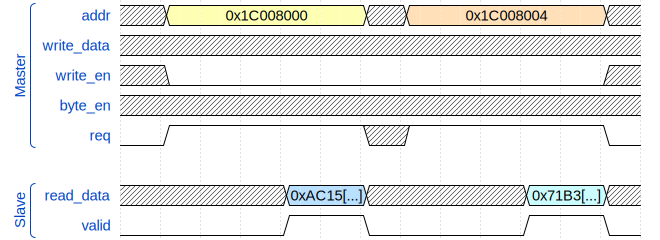
\includegraphics[width=\textwidth]{graphics/EduSoC_Bus_Read.svg}
    \vspace{-1em}
    \caption{Example Read Waveform}
    \label{fig:read_waveform}
\end{figure}
\begin{figure}[h!]
    \vspace{1em}
    \centering
    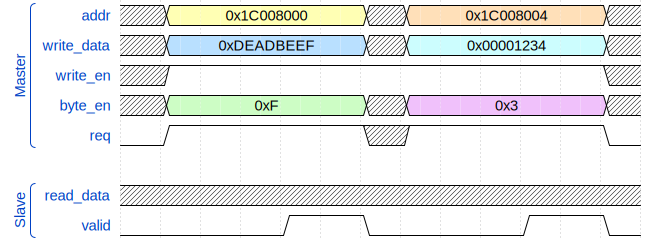
\includegraphics[width=\textwidth]{graphics/EduSoC_Bus_Write.svg}
    \vspace{-1em}
    \caption{Example Write Waveform}
    \label{fig:write_waveform}
\end{figure}

\subsection{Interrupt Bus}\label{sec:intbus}
The EduSoC interrupt bus has the following signals:\\
\begin{table}[H]
    \centering
    \begin{tabular}{|c|c|c|}\hline
        Name & Width (bits) & Direction \\\hline\hline
        \ttt{irq} & 1 & Generator $\Rightarrow$ Handler \\
        \ttt{irq\_id} & 5 & Generator $\Rightarrow$ Handler \\
        \ttt{irq\_ack} & 1 & Handler $\Rightarrow$ Generator \\
        \ttt{irq\_ack\_id} & 5 & Handler $\Rightarrow$ Generator \\\hline
    \end{tabular}
    \caption{Interrupt Bus Signals}
    \label{tab:intbus_signals}
\end{table}
\begin{itemize}
    \item \ttt{irq}: Set high (1) by the generator when an interrupt has occurred. Held until the interrupt is is acknowledged by the handler.
    \item \ttt{irq\_id}: When \ttt{irq} = 1, conveys the ID of the interrupt to be handled (see Section \ref{sec:interrupts}).
    \item \ttt{irq\_ack}: Set high (1) by the handler to signal that the currently asserted interrupt has been acknowledged and is being handled.
    \item \ttt{irq\_ack\_id}: When \ttt{irq\_ack} = 1, conveys the ID of the interrupt that is being acknowledged.
\end{itemize}

\subsection{SoC Interface}\label{sec:socinterface}
The SoC interface, consisting of the I/O interface and the CPU core interface, has the following signals and buses:\\
\begin{table}[H]
    \centering
    \begin{tabular}{|c|c|c|}\hline
        Name & Type or width (bits) & Direction \\\hline\hline
        \ttt{ext\_clk} & 1 & SoC input \\
        \ttt{ext\_resn} & 1 & SoC input \\
        \ttt{vga\_hsync} & 1 & SoC output \\
        \ttt{vga\_vsync} & 1 & SoC output \\
        \ttt{vga\_r} & 4 & SoC output \\
        \ttt{vga\_g} & 4 & SoC output \\
        \ttt{vga\_b} & 4 & SoC output \\
        \ttt{uart\_rx} & 1 & SoC input \\
        \ttt{uart\_tx} & 1 & SoC output \\
        \ttt{gpio\_in} & $N$ & SoC input \\
        \ttt{gpio\_out} & $N$ & SoC output \\
        \ttt{gpio\_drive} & $N$ & SoC output \\
        \ttt{pwm} & $M$ & SoC output \\
        \ttt{core\_clk} & 1 & SoC output \\
        \ttt{core\_res} & 1 & SoC output \\
        \ttt{control\_flags} & 16 & SoC output \\
        \ttt{instr\_bus} & Memory Bus & SoC is slave \\
        \ttt{data\_bus} & Memory Bus & SoC is slave \\
        \ttt{core\_int\_triggers} & 16 & SoC input \\
        \ttt{int\_bus} & Interrupt Bus & SoC is generator \\\hline
    \end{tabular}
    \caption{SoC Interface Signals}
    \label{tab:interface_signals}
\end{table}
The following are central control signals for the system and must be connected. In a simulation environment, they may be left open, as they are driven automatically.
\begin{itemize}
    \item \ttt{ext\_clk}: Externally supplied clock signal. Must be driven by a 100 MHz clock.
    \item \ttt{ext\_resn}: External reset (active low). Must be held high (1) and may optionally be asserted low (0) to reset the core and SoC.
\end{itemize}
Next is the VGA video output. For more information about these signals, see Section \ref{sec:vga}.
\begin{itemize}
    \item \ttt{vga\_hsync}: VGA horizontal sync signal.
    \item \ttt{vga\_vsync}: VGA vertical sync signal.
    \item \ttt{vga\_r}: VGA red color signal (16 levels).
    \item \ttt{vga\_g}: VGA green color signal (16 levels).
    \item \ttt{vga\_b}: VGA blue color signal (16 levels).
\end{itemize}
The following is the UART interface for external control and programming of the SoC. See Section \ref{sec:uart} for more information.
\begin{itemize}
    \item \ttt{uart\_rx}: UART receive line (to SoC).
    \item \ttt{uart\_tx}: UART transmit line (from SoC).
\end{itemize}
The following is the GPIO interface, with bit width $N = 32 \cdot \text{\#ports} \leq 512$. The three signals are designed to be combined into a single $N$-bit bidirectional I/O port. For more information, see Section \ref{sec:per_gpio}.
\begin{itemize}
    \item \ttt{gpio\_in}: GPIO input signals.
    \item \ttt{gpio\_out}: GPIO output signals.
    \item \ttt{gpio\_drive}: GPIO driver controls. If a bit is 0, that pin of the port is an input (``high impedance''), reading from the corresponding \ttt{gpio\_in} bit. If a bit is 1, that pin of the port is an output, writing to the corresponding \ttt{gpio\_out} bit.
\end{itemize}
The following is the output for the PWM modules, containing $M$ pulse width modulated signals, where $M \leq 16$ is the number of PWM modules in the SoC. See Section \ref{sec:per_pwm} for more information.
\begin{itemize}
    \item \ttt{pwm}: PWM output signals.
\end{itemize}
Finally, the following is the CPU core interface. See Sections \ref{sec:membus} and \ref{sec:intbus} for the memory and interrupt bus descriptions, respectively.
\begin{itemize}
    \item \ttt{core\_clk}: CPU core clock.
    \item \ttt{core\_res}: CPU core reset, active high. Intended as a synchronous reset, so the core should be reset on the rising edge of \ttt{core\_clk} if this signal is high (1).
    \item \ttt{control\_flags}: User definable control signals for the core. See Section \ref{sec:per_control} for more information.
    \item \ttt{instr\_bus}: CPU instruction memory bus. Intended to be used by the core to load program instructions from memory.
    \item \ttt{data\_bus}: CPU data memory bus. Intended to be used by the core to read and write memory or peripheral register values.
    \item \ttt{core\_int\_triggers}: Core interrupt triggers. If asserted high, a corresponding interrupt will be triggered. See Section \ref{sec:interrupts} for more information.
    \item \ttt{int\_bus}: CPU interrupt bus.
\end{itemize}